\documentclass[11pt, aspectratio = 169]{beamer}

\usetheme[progressbar=frametitle]{metropolis}
\usepackage{appendixnumberbeamer}
\usepackage{booktabs}
\usepackage[scale=2]{ccicons}
\usepackage{pgfplots}
\usepgfplotslibrary{dateplot}
\usepackage{xspace}
\usepackage{hyperref}
\usepackage{verbatim} 
\newcommand{\themename}{\textbf{\textsc{metropolis}}\xspace}
\definecolor{links}{HTML}{1B1B81}
\hypersetup{colorlinks,linkcolor=blue,urlcolor=blue}

% listings: To highlight code:
\usepackage{listings}
\lstset{
  language=R,
  basicstyle=\ttfamily\footnotesize,
  keywordstyle=\color{blue},
  commentstyle=\color{green!50!black},
  stringstyle=\color{red},
  frame=single,
  showstringspaces=false
}
\lstset{basicstyle=\ttfamily\footnotesize, frame=single}

% To comment out large sections:
\usepackage{comment}

\title{Applied Economics}
\subtitle{Statistical Inference I}
\author{Pello Aspuru}
\date{}
\institute{Winter 2025/26}
% \titlegraphic{\hfill\includegraphics[height=1.5cm]{logo.pdf}}
\setbeamercolor{normal text}{fg=black}
\setbeamercolor{block title}{fg=teal}
\setbeamercovered{transparent} % default faintness (~15%)

\let\svdescription\description
\let\svenddescription\enddescription
\renewenvironment{description}{%
  \svdescription%
  \let\svitem\item%
  \renewcommand\item[1][]{\svitem[\textcolor{\descriptioncolor}{##1}]}%
  }{
  \svenddescription%
  }
\newcommand\descriptioncolor{teal}

%\usepackage{Sweave}
\begin{document}
%\input{AE_w5_inference-concordance}

\maketitle

\begin{frame}{Big Picture: Steps in empirical economic analysis}
    \begin{center}
        Economic question: does education \alert{cause} an increase in wages?
    \end{center}
    \vspace{-3mm}
\pause
\vspace{+0.2cm}
\begin{enumerate}
    \item Construct an economic model for the \alert{representative agent}.
        $$wage = \beta_0 + \beta_1 educ + \beta_2 expert + \beta_3 is\_female $$
    \vspace{-4mm}
    \item Turn the economic model into a statistical model for the \alert{population}.
        $$wage_{it} = \beta_0 + \beta_1 educ_{it} + \beta_2 expert_{it} + \beta_3 is\_female_{it} + \alert{u_{it}} \quad i=1,...,N$$
    \pause
    \vspace{-4mm}
    \item Turn the statistical model for the \alert{observed sample}.
        $$wage_{it} = \hat{\beta}_0 + \hat{\beta}_1 educ_{it} + \hat{\beta}_2 expert_{it} + \hat{\beta}_3 is\_female_{it} + \alert{\hat{u}_{it}} \quad i=1,...,n$$
    \pause
    \vspace{-4mm}
    \item Formulate conjectures (hypothesis) about the parameter of interest $\beta_1$. 
    \begin{itemize}
        \item e.g. education causes an increase in wage $\rightarrow$ $\beta_1 >0$. 
        \item Can we answer this question without observing $\beta_1$?  
    \end{itemize}
\end{enumerate}
\end{frame}

\begin{frame}{Roadmap}
\begin{block}{Statistical Inference}
    Use the vector of parameter estimates $\hat{\beta}$ and standard error matrix $\widehat{SE}(\hat{\beta})$ to infer about the true parameter $\beta_1$
\end{block}
\pause
\begin{enumerate}
    \item Hypothesis tests for a single population parameter
    \begin{itemize}
        \item Two-sided tests
        \item One-sided tests
    \end{itemize}
    \item confidence intervals of parameter estimates \pause
    \item Hypothesis tests for a multiple population parameter (next session)
   % \item multiple hypothesis tests
\end{enumerate}
\pause 
To make inference about the unknown population parameters, we will use: 
\begin{itemize}
    \item the OLS estimator $\hat{\boldsymbol{\beta}}$,
    \item its variance estimator $\widehat{Var}(\boldsymbol{\hat{\beta}|X})$,
    \item and its asymptotic distribution $N(\boldsymbol{\beta},  Var(\boldsymbol{\hat{\beta}|X}))$
\end{itemize}
\end{frame}

\section{t-tests for single coefficients}

\begin{frame}{Two-Sided Hypothesis Tests: Intuition}
\vspace{+0.2cm}
Hypothesis in a \alert{two-sided} t-test: 
\begin{align*}
    H_{0}\text{:}\: \beta_j = \beta_{j,0} \:\: \text{  vs.  } \:\: H_1\text{:}\: \beta_j \neq \beta_{j,0} 
\end{align*}
\pause 
Intuition of Hypothesis Testing:
\begin{enumerate}
\item According to the null hypothesis ($H_0$), OLS parameter estimate $\hat{\beta}_j$ features an asymptotically normal distribution centered at $\beta_{j,0}$, with variance $var(\hat{\beta}_j)$.
\item  Based on data $(X,Y)$, observe a single realization of $\hat{\beta}_j$.
\item  Assess if the parameter estimate $\hat{\beta}_j$ is likely to come from a normal distribution centered at $\beta_{j,0}$, with variance $var(\hat{\beta}_j)$.
\pause
\item Or, equivalently, if $\frac{\hat{\beta}_j - \beta_{j,0}}{sd(\hat{\beta}_j)}$ is asymptotically N(0,1)-distributed.
\end{enumerate}
\end{frame}

\begin{frame}{T-Statistic for Hypothesis Testing}
\begin{block}{Test Statistic $T_{\beta_j}$}
    \begin{align*}
    \frac{\hat{\beta}_j - \beta_{j,0}}{\alert{sd(\hat{\beta}_j)}} \quad \rightarrow \quad
    T_{\beta_j} = \frac{\hat{\beta}_j - \beta_{j,0}}{\widehat{SE}(\hat{\beta}_j)}
    \end{align*}
    One can show that, if we replace the \alert{unknown $sd(\hat{\beta}_j)$} with our consistent estimate $\widehat{SE}(\hat{\beta}_j)$, the resulting t-statistic is also asymptotically N(0,1)-distributed.
\end{block}
\pause
$\rightarrow$ According to the null hypothesis $H_0$, we know that $T_{\beta_j}$ is approximately standard normal in finite but \textbf{large samples} (given MLR.1 to MLR.4).

%\color{gray} Alternative: assume normally distributed errors (MLR.6) $\rightarrow$ test statistic follows a $t$-distribution with $n-k-1$ degrees of freedom
\end{frame}

\begin{frame}[fragile]{Two-Sided Hypothesis Test: Procedure}

Is the effect of education on wages $\beta_1 = 0.8$? \pause $H_{0}\text{:}\: \beta_1 = 0.8 \:\: \text{  vs.  } \:\: H_1\text{:}\: \beta_1 \neq 0.8$
\pause
\begin{enumerate}
    \item Specify a significance level $\alpha$, e.g. $\alpha = 5\%$.
    \item $Q_{\alpha}$ is the $c = (1-\alpha/2)$-quantile from the N(0,1) distribution.
    \begin{lstlisting}[language=R]
    alpha <- 0.05
    Q_alpha <- qnorm(1-alpha/2)
    \end{lstlisting}
    \pause
    \item Compute the Test-statistic realization: $T_{\beta_j} = \frac{\hat{\beta}_j - \beta_{j,0}}{\widehat{SE}(\hat{\beta}_j)}$. e.g. $T_{\beta_1} = -3.09$.
    \vspace{3mm}
    \begin{lstlisting}[language=R]
    T_educ <- (beta_hat_educ-0.8)/SE_hat_educ
    \end{lstlisting} \pause
    \item If $| T_{\beta_j} | > Q_{\alpha}$ is true, Reject null hypothesis $\beta_1 = 0.8$, with $1-\alpha$ probability.
    \vspace{3mm}
    \begin{lstlisting}[language=R]
    abs(T_educ) > Q_alpha
    \end{lstlisting} \pause
    \item[$\rightarrow$] $\alpha$ is the probability to reject $H_0$ if it is true (Type I error).
\end{enumerate}
\end{frame}

\begin{frame}[fragile]{Two-Sided Hypothesis Test: Special Case}
    The most common two-sided tests consists on whether $\beta_j$ is zero:
    $$H_{0}\text{:}\: \beta_1 = 0 \:\: \text{  vs.  } \:\: H_1\text{:}\: \beta_1 \neq 0$$
    R features default function \texttt{coeftest()} for this hipothesis testing:
    \begin{enumerate}
        \item Estimate multiple linear regression model, find vector $\hat{\beta}$.
        \begin{lstlisting}[language=R]
        mlr <- lm(wage ~ educ + exper +  female, data = df_wages)
        \end{lstlisting}
        \item Retrieve robust empirical variance matrix $\widehat{Var}(\hat{\beta}|X)$
        \begin{lstlisting}[language=R]
        robust_vcov <- vcovHC(mlr, type = "HC0")
        \end{lstlisting}
        \pause
        \item Test whether each element in $\hat{\beta}$ is different from zero.
        \begin{lstlisting}[language=R]
        coeftest(fit, vcov = robust_vcov)
        \end{lstlisting}
        \item Reports $t_{\beta_j} = \frac{\hat{\beta}_j - 0}{\widehat{SE}(\hat{\beta}_j)}$ for each parameter estimate.
    \end{enumerate}
\end{frame}

\begin{comment}
    \begin{frame}{Critical Value / Critical Region}
\begin{figure}
    \centering
      \only<1>{ 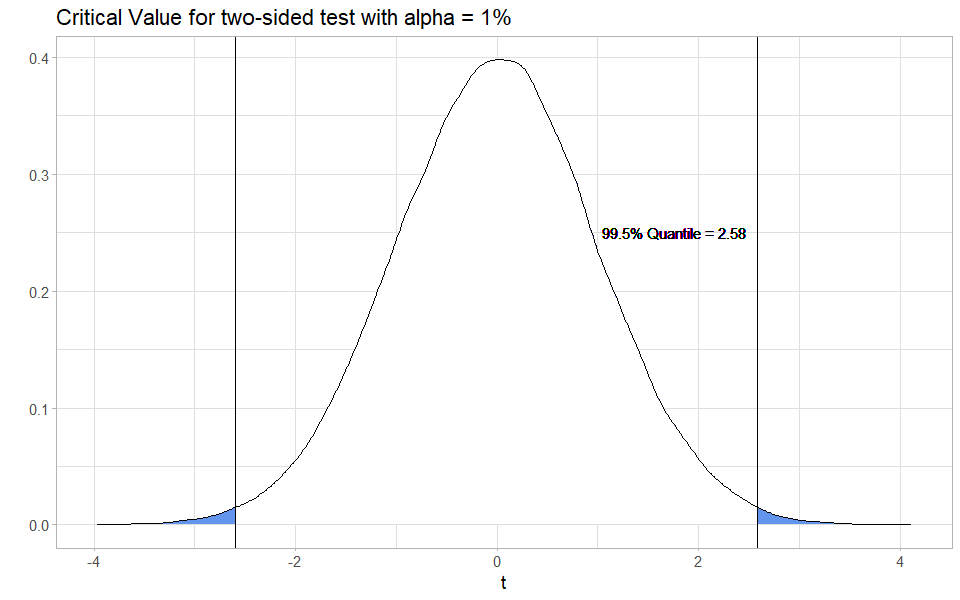
\includegraphics[width = .85\linewidth]{plot3.png}}
  \only<2>{ 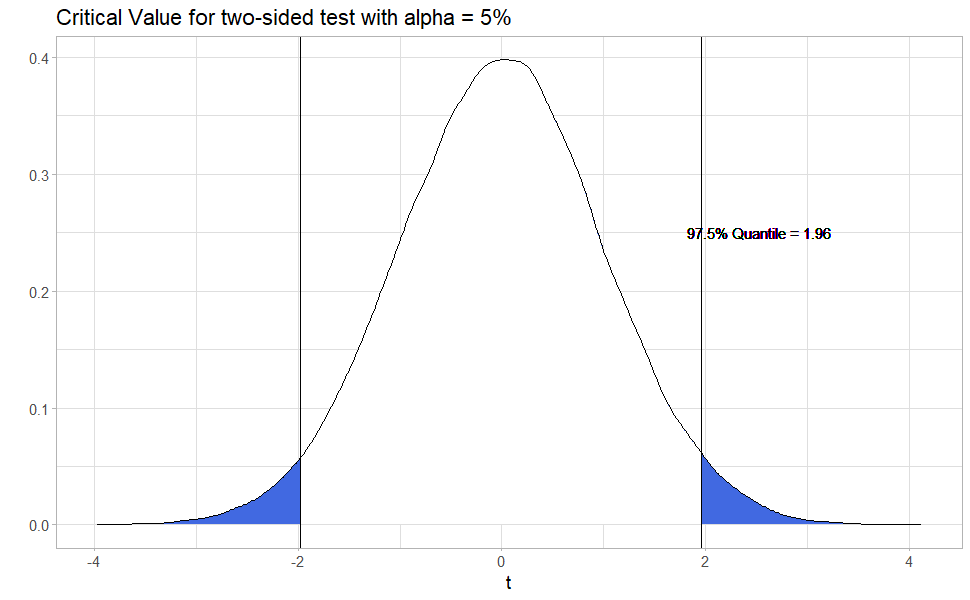
\includegraphics[width = .85\linewidth]{plot1.png}}
    \only<3>{ 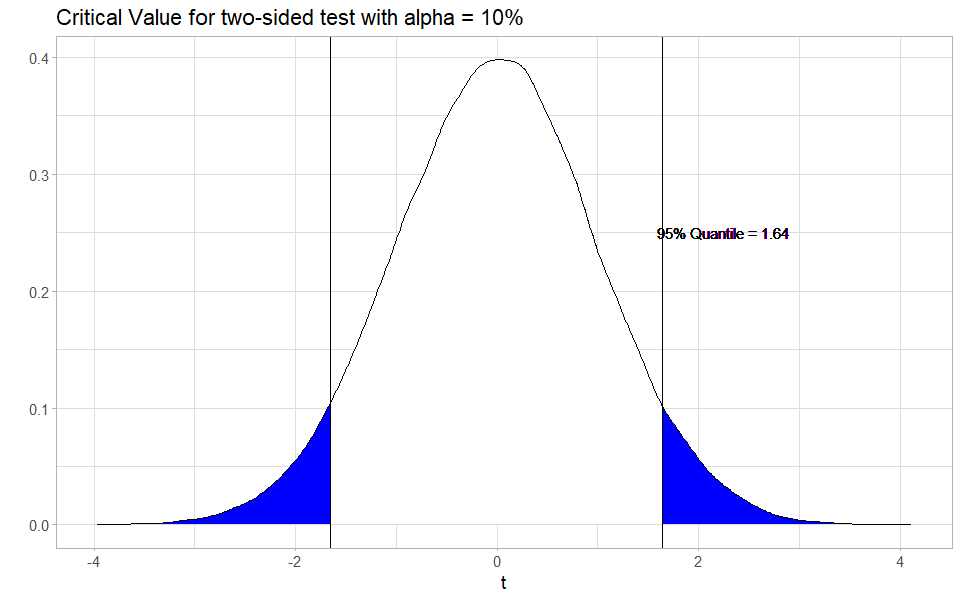
\includegraphics[width = .85\linewidth]{plot2.png}}
    \label{fig:enter-label}
\end{figure}
\end{frame}
\end{comment}

\begin{frame}[fragile]{One-sided t-Test}
Is the effect of education on wages larger than 0.1?
\begin{align*}
    H_0\text{:} \: \beta_1 \geq 0.1 \: \text{  vs.  } \: H_1\text{:} \: \beta_1 < 0.1 
\end{align*}

\begin{enumerate}
    \item Specify a significance level $\alpha$ $\rightarrow$ $Q_{\alpha}$ is the $\alpha$-quantile from N(0,1).
    \begin{lstlisting}[language=R]
    Q_alpha <- qnorm(alpha)
    \end{lstlisting}
    \pause
    \item Compute the Test-statistic realization: $T_{\beta_j} = \frac{\hat{\beta}_1 - 0.1}{\widehat{SE}(\hat{\beta}_1)}$.
    \vspace{3mm}
    \begin{lstlisting}[language=R]
    T_educ <- (beta_hat_educ-0.1)/SE_hat_educ
    \end{lstlisting} \pause
    \item If $| T_{\beta_j} | > Q_{\alpha}$ is true, accept null hypothesis $\beta_1 \geq 0.8$, with $1-\alpha$ probability.
    \vspace{3mm}
    \begin{lstlisting}[language=R]
    abs(T_educ) > Q_alpha
    \end{lstlisting} \pause
    \item[$\rightarrow$] How should the previous procedure change to test $H_0\text{:} \: \beta_1 \leq 0.1$ ?
\end{enumerate}
\end{frame}

\begin{comment}
    \begin{frame}{Critical Value / Critical Region}
\begin{figure}
    \centering
      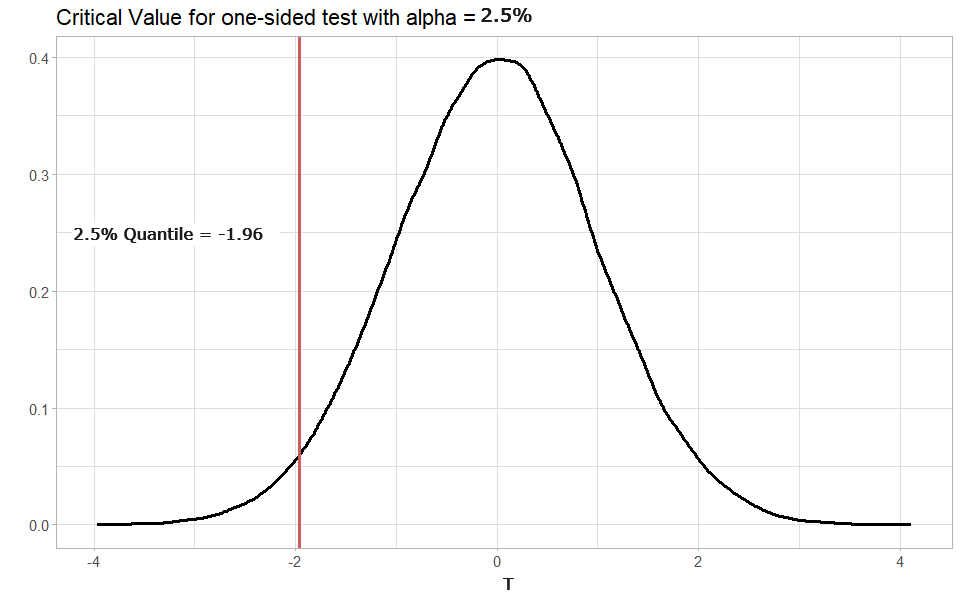
\includegraphics[width = .85\linewidth]{plot4.png}
\end{figure}
\end{frame}
\end{comment}

\begin{frame}{Recap: Hypothesis Tests}    
With our result on asymptotic normality of the OLS estimator and a hypothesis we want to test, we can construct a \textbf{test-statistic with known distribution under $H_0$.} 

We compare the realization in our sample to a \textbf{critical value} that is derived based on a pre-specified significance level and the distribution under $H_0$.

We reject the null (find evidence for the alternative), if the realized test statistic is very unlikely under $H_0$, i.e. inconsistent with the distribution under $H_0$.
\end{frame}

\section{p-values}
\begin{frame}[fragile]{p-value: Definition}
The \textbf{p–value} is the \alert{smallest} significance level $\alpha$ at which the hypothesis test would be rejected.
\pause
\begin{lstlisting}[language=R]
    coeftest(mlr, vcov = robust_vcov)
\end{lstlisting}
\begin{itemize}
    \item[$\rightarrow$] 0.04288 means that there is a 4.288\% probability $\beta_0=0$.
\end{itemize}
\end{frame}

\begin{comment}
    \begin{frame}{p-value: Illustration}
\begin{figure}
    \centering
      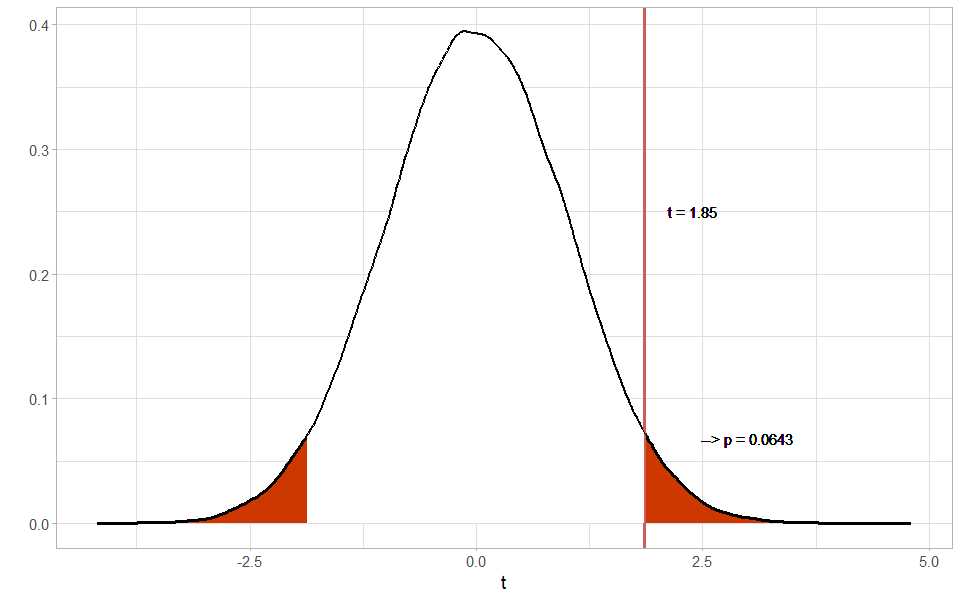
\includegraphics[width = .85\linewidth]{plot5.png}
\end{figure}
\end{frame}
\end{comment}

\begin{frame}{p-value}
Communicating statistical significance based on p-values (or test statistics) provides more information than only reporting one specific test decision.

e.g. ''the p-value on coefficient $\beta_0$ is 0.04288'' vs. ''the null $H_0: \beta_0 = 0$ is rejected at the 5\% level.'' 
\vspace{+0.4cm}
\pause
\begin{block}{Statistical vs. Economic Significance}
  \begin{itemize}
      \item $t$-test/$p$-value on $\beta_j$ informs us about $X_j$'s \textit{statistical} significance for $Y$ $\rightarrow$ does it make sense to interpret the coefficient at all, given the estimation uncertainty?
\item Whether the regressor has an \textit{economically relevant} impact on $Y$ depends on the \textit{size} of the coefficient.

\item To interpret the size, computing the effect of a st.dev.-change in $X_j$ can be helpful.
  \end{itemize}  
\end{block}
\end{frame}



\begin{frame}[fragile]{Examples}

\begin{itemize}
    \item Run model with logs of wages as dependent variable. Why?
    \begin{lstlisting}[language=R]
    mlr_2 <- lm(log(wage) ~ educ + exper +  female, data = df_wages)
    robust_vcov_2 <- vcovHC(mlr_2, type = "HC0")
    \end{lstlisting}
    \item Retrieve $\hat{\beta}_1$ parameter estimate of interest, with corresponding standard error.
    \begin{lstlisting}[language=R]
    beta_educ      <- coef(mlr_2)["educ"]
    se_educ_robust <- sqrt(diag(robust_vcov_2))["educ"]
    \end{lstlisting}
    \item Estimate the effect of a +1 standard deviation of education attainment on wage.
    \begin{lstlisting}[language=R]
    sd_educ        <- sd(df_wages$educ, na.rm = TRUE)
    effect_1sd      <- beta_educ * sd_educ
    \end{lstlisting}
\end{itemize}
\pause
    \texttt{effect\_1sd} $\approx$ 0.25\% $\rightarrow$ A st.dev. increase in education increases the wage by 25\%.
\end{frame}

\section{Confidence Intervals}

\begin{frame}[fragile]{Confidence Intervals}

\begin{block}{Confidence Intervals (CI)}
    provide a lower and an upper bound (both are random variables!) on ''likely'' values for $\beta_j$ , and thus an idea of the precision of the estimation.
\end{block}
\pause
CIs  are computed for a pre-specified confidence level $(1-\alpha)$ as:
$$\widehat{CI}(\beta_j) = [\hat{\beta_j}\alert{-}c_{1-\alpha/2}\color{black} \cdot SE(\hat{\beta_j}) \quad ; \quad \hat{\beta_j}\alert{+} c_{1-\alpha/2}\color{black}\cdot SE(\hat{\beta_j})]$$
\pause
This is the critical value $c$ from a two-sided t-test at significance level $\alpha$.
\begin{lstlisting}[language=R]
    coefci(mlr, vcov = robust_vcov)
\end{lstlisting}
\pause
\begin{itemize}
    \item The (1$-\alpha$)$-$CI of $\beta_j$ satisfies:  $Pr(\beta_j \in \widehat{CI}(\beta_j) ) = 1 – \alpha$
    \item[$\rightarrow$] For $\alpha=5\%$, there is a 95\% probability that $\beta_1 \in [0.477, 0.728]$ 
\end{itemize}
\end{frame}

\begin{frame}{Confidence Intervals}

\begin{itemize}
    \item Interpretation: With probability $(1 – \alpha)$\% the CI covers the true $\beta_j$. 
    \item If we would draw several samples from the population and compute $\widehat{CI}(\beta_j)$ for each sample, $(1 – \alpha)$\% of all intervals would include the true $\beta_j$.
    \item Relation to hypothesis test at level $\alpha$: \\
    If the (1$-\alpha)-$CI for $\beta_j$ does not contain $\beta_{j,0}$, we reject $H_0: \beta_j = \beta_{j,0}$ at significance level $\alpha$.
\end{itemize}
 
\end{frame}

\begin{frame}[fragile]{Visualizing Confidence Intervals in R}
Lets make a plot with the 95\% confidence intervals of $\beta$ parameters.
\pause
\begin{enumerate}
    %\item run script \texttt{session5.R} from moodle.
    \item store the results from \texttt{coefci(...)} as confidence interval matrix \texttt{ci\_mat}.
    \item Arrange \texttt{ci\_mat} as a tidy dataset \texttt{df\_ci}.
    \pause
    \item use \texttt{ci\_mat} as input for \texttt{ggplot()} function:
    \begin{lstlisting}[language=R]
    ggplot(df_ci, aes(x = term, y = estimate)) +
    geom_hline(yintercept = 0, linetype = "dashed") +
    geom_pointrange(aes(ymin = conf.low, ymax = conf.high))
    \end{lstlisting}
    \pause
    \item Make aesthetic changes:
    \begin{lstlisting}[language=R]
    labs(x = NULL,
         y = "Coefficient (robust 95% CI)",
         title = "Robust (HC0) Confidence Intervals from lm") +
         theme_minimal(base_size = 12)
    \end{lstlisting}
\end{enumerate}
\end{frame}

\begin{frame}{Plot}
\begin{center}
    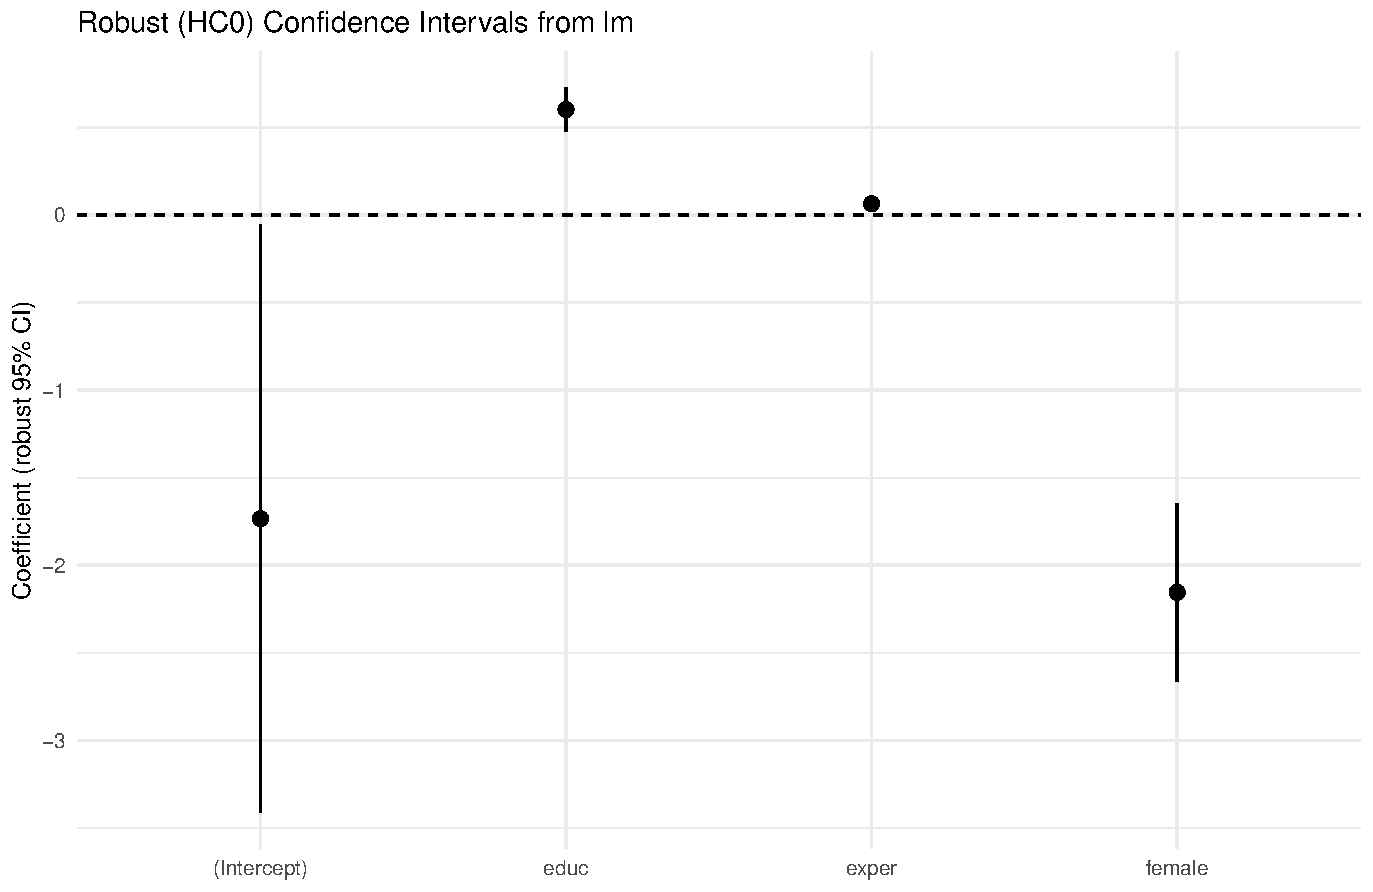
\includegraphics[width = .7\linewidth]{conf_int_plot.pdf}
\end{center}
\end{frame}
%\section{multiple hypotheses tests}

\begin{frame}
See \alert{w5\_code.R} for the complete code.
\end{frame}
\end{document}





